\chapter{Implementation and Evaluation}

\section{Wrapping MonPoly}

The wrapper runs MonPoly as a subprocess and handles all interactions with MonPoly itself.
Incoming events are first parsed and checked on some major formatting errors.
When the formatting is deemed acceptable the events get forwarded to MonPoly on a per time point basis.
If MonPoly reports an issue with a certain time stamp, either it is out of order or one event at that timestamp does not comply with the given signature, this time stamp gets ignored by MonPoly, and in turn the wrapper discards it as well.
If no issue is detected with a timestamp all events in at that timestamp get forwarded to the database.
Figure \ref{fig:flowchart} illustrates the control flow of this process.

\subsection{Flask}
Flask \cite{Flask} is a lightweight web framework for Python.




\section{Policy Change}
% \tikzstyle{startstop} = [rectangle, rounded corners, 
minimum width=3cm, 
minimum height=1cm,
text centered, 
draw=black]
% fill=red!30]

\tikzstyle{io} = [trapezium, 
trapezium stretches=true, % A later addition
trapezium left angle=70, 
trapezium right angle=110, 
minimum width=3cm, 
minimum height=1cm, text centered, 
draw=black]
% , fill=blue!30]

\tikzstyle{process} = [rectangle, 
minimum width=3cm, 
minimum height=1cm, 
text centered, 
text width=3cm, 
draw=black] 
% fill=orange!30]

\tikzstyle{decision} = [diamond, 
minimum width=2cm, 
minimum height=1cm, 
text centered, 
text width=3cm,
draw=black]
% fill=green!30]
\tikzstyle{arrow} = [thick,->,>=stealth]

\begin{tikzpicture}[node distance=2cm]

% \node (start) [startstop] {Start};
% \node (in1) [io, below of=start] {Events get sent to wrapper};
\node (in1) [io] {Events get sent to wrapper};
\node (pro1) [process, below of=in1] {Wrapper checks JSON formatting};
\node (dec1) [decision, below of=pro1, yshift=-1.5cm] {JSON formatting correct?};

\node (pro2a) [process, below of=dec1, yshift=-2cm] {Convert JSON input to list of MonPoly style log strings for each time point};
\node (pro2b) [io, right of=dec1, xshift=3.2cm] {Abort and report issue to user};
\node (pro3) [process, below of=pro2a] {Send next time point to MonPoly};
\node (dec2) [decision, below of=pro3, yshift=-2cm] {Time point in order and predicates comply with signature?};
% \node (stop) [startstop, below of=pro3]{Stop};

% \draw [arrow] (start) -- (in1);
\draw [arrow] (in1) -- (pro1);
\draw [arrow] (pro1) -- (dec1);
\draw [arrow] (dec1) -- node[anchor=east] {yes} (pro2a);
\draw [arrow] (dec1) -- node[anchor=south] {no} (pro2b);
\draw [arrow] (pro2a) -- (pro3);
\draw [arrow] (pro3) -- (dec2);

\end{tikzpicture}

\begin{figure}
    \label{fig:flowchart}
    \centering
    % 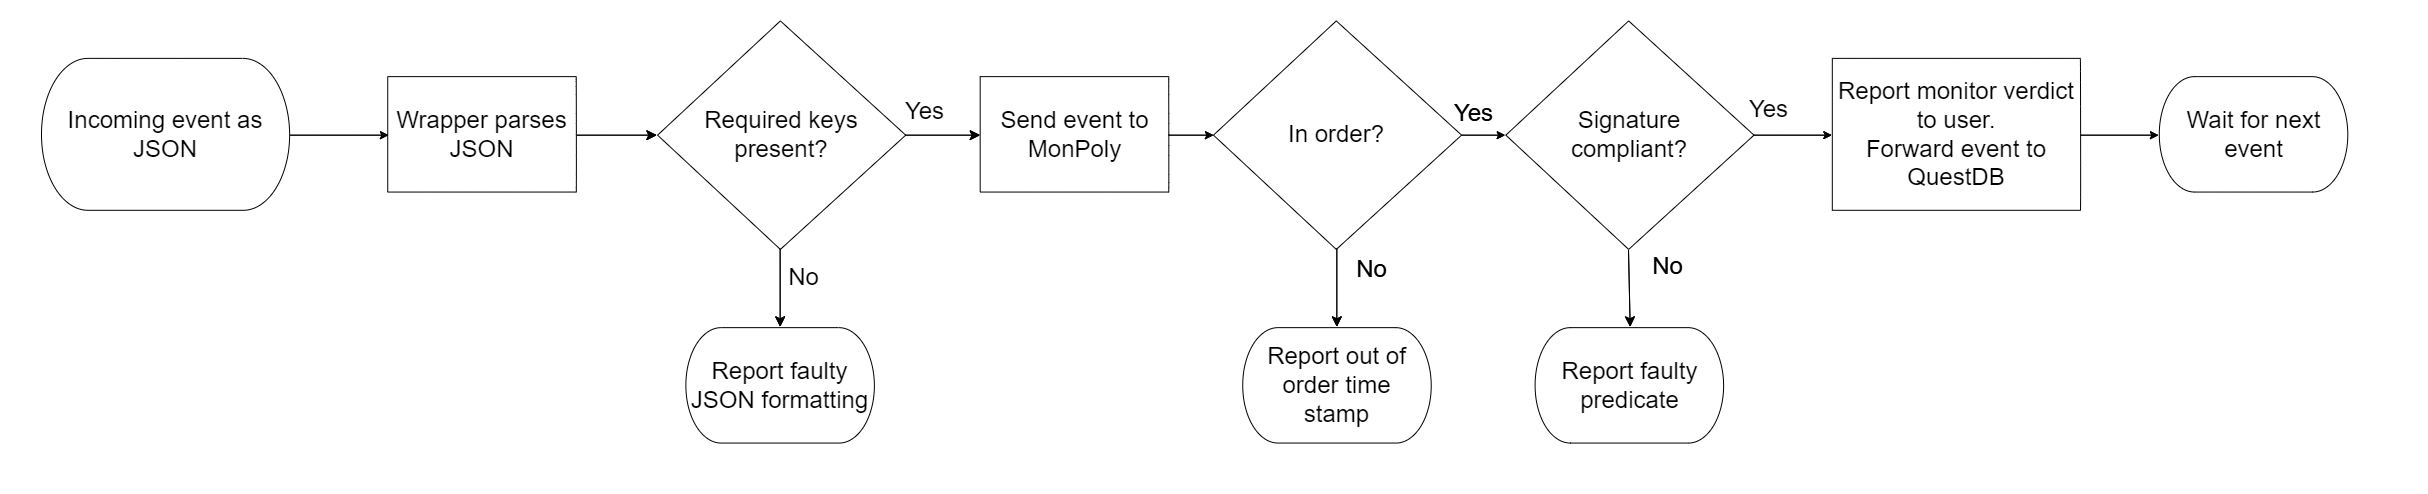
\includegraphics[width=110mm]{diagrams/flowchart.png}
    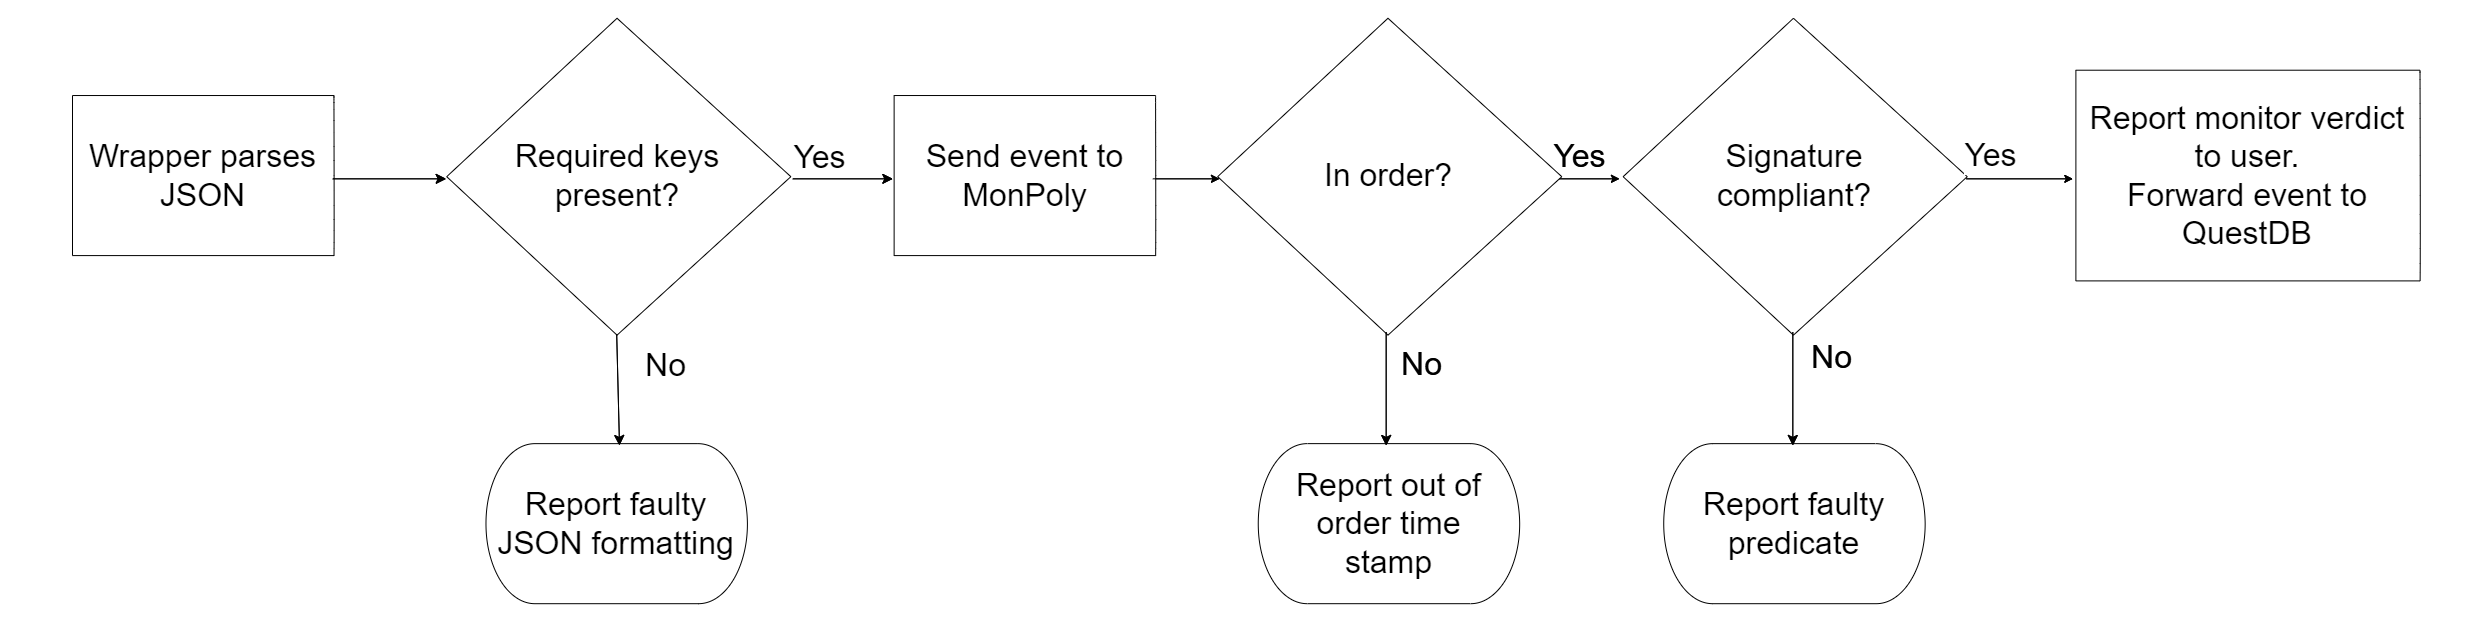
\includegraphics[width=\linewidth]{diagrams/flowchart-2.png}
    \caption{Control flow for a new event}
\end{figure}

The naive approach to a policy change is sipmly reloading all events that have ever been seen by the monitor and in turn are in the database.

This first version of a policy change functions by stopping the current monitor and starting a new one.
When starting the new monitor we want to restore the state of the old one.
We do this by querying old events from our database.
But we do not simply query for the entirety of the database.
We make two optimizations.
First we use relative intervals and second we make use of constant values.
For each predicate occurring in a formula we look for constant attributes in its occurrences.
For every predicate and its potential occurrences with different constant values we then compute an over approximation of the relative interval.
We use this information to create a SQL query that only queries the constant values combined with the interval.
This way we minimize the amount of data that the new monitor has to read and process.

\section{Performance Overhead}


\section{Partial Policy Change}

We have started looking into a different method for a policy change that could be done directly through MonPoly and would not rely on the wrapper and the presence of a database.
The general idea is that in many use cases it is common that a policy is made up of many individual parts and one might want to change only a small part of a formula.
Consider for example a privacy policy on a website.
Let's say a user has the ability to specify where their data may and may not be used.
Maybe they had selected very restrictive options, but now want to allow their data to be used in one specific case.
MonPoly has now continuously been monitoring the restrictive policy and also has the state for all the sub-formulas in the larger policy.
In terms of efficiency it would be useful, if the state would only need to be recomputed for the one part that got changed and if the rest of the state could be kept.

One case might be where policies are all in conjunctive normal form (CNF) and single conjuncts might get added or removed.
To remove a conjunct from the formula it needs some sort of identifier.
In a regular structure like a CNF formula this could be done by automatic indexing.
But it still poses some questions, like what happens if the monitor rewrites the formula to an equivalent one, but changes the order.
Then the user doesn't have an inherent idea of a conjuncts' location anymore.
Our solution to this problem was thus to let the user provide identifiers in the form of strings for certain sub-formulas.

We have begun implementing this change in MonPoly.
Our idea makes use of the existing commands feature that lets a user control certain aspects of MonPoly during its runtime.
We envision commands of the form "remove sub-formula x", "add formula y as a conjunct to sub-formula x".
The second example would replace place the sub formula "x and y" in place of "x".
An analogous thing for "or" with an "add disjunct" command is also perceivable.
Or also a command like "negate sub-formula x".

With all this, MonPoly would parse the new formula part, add it to the existing formula, check if the new formula is monitorable, and if so it updates the policy.
Similarly if a part gets removed a check on monitorability of the remaining formula needs to be done.
Before adding a sub-formula, the existing trace has to be checked against that sub-formula and this state must get combined with the pre-existing state of MonPoly.

We have started implementing a feature that allows for named formulas inside MonPoly.
The names should have no effect on the monitoring and solely act as the identifiers of formula parts.

